\documentclass[11pt,a4paper]{article}
\usepackage[utf8]{inputenc}
\usepackage[T1]{fontenc}
\usepackage{lmodern}
\usepackage[french]{babel}
\usepackage{amsmath,amssymb,amsthm}
\usepackage[margin=2.5cm]{geometry}
\usepackage{xcolor}
\usepackage{graphicx}
\newtheorem*{theorem*}{Théorème}

\newtheorem{remarque}{Remarque}
\newcommand{\sign}{\operatorname{sign}}
\newcommand{\hth}{\hat{\theta}}
\newcommand{\hw}{\hat{\omega}}

\title{Estimation de la position du réseau par PLL\\ à mode glissant d'ordre deux (Super-Twisting)}
\author{}
\date{}

\begin{document}
\maketitle

\section{Tensions du réseau et transformation de Clarke}

On considère un réseau triphasé équilibré, écrit avec la convention cosinus :
\begin{align}
V_a &= V_m \cos\theta, \\
V_b &= V_m \cos\!\left(\theta - \tfrac{2\pi}{3}\right), \\
V_c &= V_m \cos\!\left(\theta + \tfrac{2\pi}{3}\right),
\end{align}
avec $\theta = \omega t + \theta_0$.

La transformation de Clarke (version invariante en amplitude) donne
\begin{align}
V_\alpha &= \frac{2}{3}\left(V_a - \frac{1}{2}V_b - \frac{1}{2}V_c\right), \\
V_\beta  &= \frac{2}{3}\left(\frac{\sqrt{3}}{2}V_b - \frac{\sqrt{3}}{2}V_c\right),
\end{align}
d'où
\begin{equation}
V_\alpha = V_m\cos\theta, \qquad V_\beta = V_m\sin\theta .
\end{equation}

\begin{remarque}
Si l'on adopte plutôt $V_a = V_m\sin\theta$, on obtient $V_\alpha = V_m\sin\theta$ et
$V_\beta = -V_m\cos\theta$. La PLL ci-dessous convergerait alors vers $\theta-\pi/2$.
Il faut donc fixer une seule convention. Un déphasage constant
$V_a = V_m\cos(\theta+\Delta\theta)$ conduit simplement à l'estimation de $\theta+\Delta\theta$.
\end{remarque}

\section{Détecteur de phase}

Soit $\hth$ la position estimée. On définit le signal d'erreur
(composante $q$ de la transformation de Park calculée avec $\hth$) :
\begin{align}
\varepsilon &= -V_\alpha\sin\hth + V_\beta\cos\hth \\
&= V_m\left[\sin\theta\cos\hth - \cos\theta\sin\hth\right] \\
&= V_m\sin(\theta-\hth) = V_m \sin\psi, \qquad \psi \triangleq \theta-\hth .
\end{align}

Pour rendre les gains indépendants de l'amplitude, on normalise :
\begin{equation}
\hat V_m = \sqrt{V_\alpha^2+V_\beta^2}, \qquad
e = \frac{\varepsilon}{\hat V_m} = \sin\psi \;\approx\; \psi \quad (|\psi|\ll 1).
\end{equation}

\section{Dynamique de l'erreur}

En supposant $V_m$ constant :
\begin{equation}
\dot\psi = \omega - \hw, \qquad \hw \triangleq \frac{d\hth}{dt},
\end{equation}
\begin{equation}
\dot e = \cos\psi\,\dot\psi = \cos\psi\,(\omega-\hw).
\end{equation}

\begin{remarque}
Le facteur $\dot\psi$ est indispensable : $\dot\varepsilon = V_m\cos\psi\,\dot\psi$, et non $V_m\cos\psi$.
De même, avec $V=\tfrac12\varepsilon^2$, on a
$\dot V = \varepsilon\dot\varepsilon = V_m^2\sin\psi\cos\psi\,(\omega-\hw)$.
\end{remarque}

\section{Loi d'estimation Super-Twisting}

On choisit
\begin{align}
\hw &= k_1 |e|^{1/2}\sign(e) + z + \omega_{ff}, \\
\dot z &= k_2 \sign(e), \\
\dot{\hth} &= \hw ,
\end{align}
où $\omega_{ff}$ est la pulsation nominale (anticipation, par ex.\ $2\pi\cdot 50$ rad/s)
et $k_1,k_2>0$.

\begin{remarque}
Les signes sont \emph{positifs} dans la loi sur $\hw$. La forme standard
$-k_1|x|^{1/2}\sign(x) + z$, $\dot z = -k_2\sign(x)$ décrit la dynamique
\emph{en boucle fermée} de l'erreur, et non la loi de commande. Comme
$\dot\psi = \omega-\hw$, appliquer les signes négatifs directement sur $\hw$
crée une rétroaction positive, et l'estimateur diverge.
\end{remarque}

\section{Analyse de stabilité détaillée}

\subsection{Hypothèses}
\begin{description}
  \item[H1] Réseau équilibré, amplitude $V_m>0$ constante (ou lentement variable), sans harmoniques.
  \item[H2] La fréquence est dérivable et sa dérivée (RoCoF) est bornée : $|\dot\omega(t)|\le L$.
  \item[H3] L'erreur initiale vérifie $|\psi(0)|<\pi/2$. L'analyse est donc \emph{locale}.
\end{description}

\subsection{Équations de l'erreur en boucle fermée}
On pose
\begin{equation}
x_1 \triangleq \psi = \theta-\hth, \qquad x_2 \triangleq (\omega-\omega_{ff}) - z .
\end{equation}
Avec $e=\sin\psi$, on a $\dot\psi=\omega-\hw$ et $\dot z = k_2\sign(e)$. Pour $|\psi|<\pi$,
$\sign(\sin\psi)=\sign(\psi)$, donc
\begin{align}
\dot x_1 &= -k_1|\sin x_1|^{1/2}\sign(x_1) + x_2, \\
\dot x_2 &= -k_2\sign(x_1) + \dot\omega(t).
\end{align}
On introduit le gain non linéaire
\begin{equation}
g(x_1) \triangleq \left|\frac{\sin x_1}{x_1}\right|^{1/2},
\qquad |\sin x_1|^{1/2} = g(x_1)\,|x_1|^{1/2}.
\end{equation}
Comme $\sin x/x \ge 2/\pi$ pour $|x|\le\pi/2$ (inégalité de Jordan),
\begin{equation}
g(x_1)\in[\gamma_m,\,1], \qquad \gamma_m = \sqrt{2/\pi}\approx 0.798, \qquad \text{pour } |x_1|\le \pi/2 .
\end{equation}
On obtient ainsi un super-twisting avec un gain incertain $g$ sur le premier terme et une
perturbation $\rho=\dot\omega$ bornée sur le second :
\begin{equation}\label{eq:bf}
\boxed{\;
\dot x_1 = -k_1\, g(x_1)\,|x_1|^{1/2}\sign(x_1) + x_2, \qquad
\dot x_2 = -k_2\sign(x_1) + \rho(t), \quad |\rho|\le L .\;}
\end{equation}
Le point d'équilibre $(x_1,x_2)=(0,0)$ correspond à $\hth=\theta$ et à $z=\omega-\omega_{ff}$,
c'est-à-dire $\hw=\omega$.

\begin{remarque}
Utiliser $\psi$ comme variable plutôt que $e$ supprime le facteur $\cos\psi$ de $\dot e$.
Toute la non-linéarité du détecteur de phase est contenue dans $g(x_1)$.
\end{remarque}

\subsection{Fonction de Lyapunov}
On pose $\phi(x_1)=|x_1|^{1/2}\sign(x_1)$ et le vecteur
\begin{equation}
\zeta = \begin{bmatrix}\phi(x_1)\\ x_2\end{bmatrix}.
\end{equation}
On choisit la fonction candidate (forme de Moreno \& Osorio) :
\begin{equation}
V(x) = 2k_2|x_1| + \tfrac12 x_2^2 + \tfrac12\big(x_2 - k_1\phi(x_1)\big)^2 = \zeta^\top P\zeta,
\qquad
P = \frac12\begin{bmatrix}4k_2+k_1^2 & -k_1\\ -k_1 & 2\end{bmatrix}.
\end{equation}
$P$ est définie positive, car $\det P = \tfrac14(8k_2+k_1^2)>0$. $V$ est continue et
définie positive. Elle est radialement non bornée et dérivable partout sauf sur l'ensemble $x_1=0$,
que les trajectoires (hors origine) ne font que traverser. On peut donc appliquer la version
non lisse du théorème de Lyapunov, comme dans Moreno \& Osorio.

\paragraph{Dérivée de $\zeta$.} Pour $x_1\neq 0$, $\dot\phi = \tfrac12|x_1|^{-1/2}\dot x_1$.
On écrit $\rho = \delta(t)\sign(x_1) = \delta(t)\,|x_1|^{-1/2}\phi(x_1)$ avec $|\delta|\le L$, et
$\sign(x_1) = |x_1|^{-1/2}\phi(x_1)$. On obtient
\begin{equation}
\dot\zeta = |x_1|^{-1/2} A(g,\delta)\,\zeta,
\qquad
A(g,\delta)=\begin{bmatrix} -\tfrac12 k_1 g & \tfrac12 \\ -(k_2-\delta) & 0\end{bmatrix}.
\end{equation}

\paragraph{Dérivée de $V$.}
\begin{equation}
\dot V = |x_1|^{-1/2}\,\zeta^\top\big(A^\top P + PA\big)\zeta = -|x_1|^{-1/2}\,\zeta^\top Q(g,\delta)\,\zeta,
\end{equation}
où le calcul (vérifié symboliquement) donne
\begin{equation}
Q(g,\delta) = \begin{bmatrix}
\tfrac{k_1}{2}\left(gk_1^2 + (4g-2)k_2 + 2\delta\right) & -\tfrac14\left((1+g)k_1^2+4\delta\right)\\[2pt]
-\tfrac14\left((1+g)k_1^2+4\delta\right) & \tfrac{k_1}{2}
\end{bmatrix}.
\end{equation}

\subsection{Conditions sur les gains}
Comme $Q_{22}=k_1/2>0$, on a $Q>0$ si et seulement si $\det Q>0$, c'est-à-dire
\begin{equation}
8k_1^2k_2(2g-1) > (1-g)^2k_1^4 + 8\delta g k_1^2 + 16\delta^2 .
\end{equation}
Le pire cas est $\delta=L$. Cette condition exige $g>1/2$, ce qui est assuré puisque $\gamma_m\approx0.798$.

\begin{theorem*}[Conditions suffisantes]
Supposons H1--H3 et $k_1>0$. Si
\begin{equation}\label{eq:k2}
\boxed{\;k_2 > \max_{g\in[\gamma_m,1]}\;
\frac{(1-g)^2k_1^4 + 8Lgk_1^2 + 16L^2}{8k_1^2(2g-1)}\;}
\end{equation}
et si la condition initiale appartient à l'ensemble $\Omega_c$ défini en \eqref{eq:omega}, alors
$(\psi,x_2)$ converge vers $(0,0)$ en temps fini et y reste malgré $\dot\omega\neq0$.
\end{theorem*}

Dans le cas idéal $g\equiv 1$ (petites erreurs, $\sin\psi\approx\psi$), on retrouve la condition simple
\begin{equation}
k_1>0,\qquad k_2 > L + \frac{2L^2}{k_1^2}.
\end{equation}

\begin{remarque}
$Q$ est affine en $(g,\delta)$, et la plus petite valeur propre d'une matrice affine est concave.
Il suffit donc de vérifier $Q>0$ aux quatre sommets $(g,\delta)\in\{\gamma_m,1\}\times\{-L,L\}$.
On obtient un test LMI simple à faire numériquement.
\end{remarque}

\subsection{Convergence en temps fini}
On note $\mu = \min_{g,\delta}\lambda_{\min}\!\big(P^{-1/2}QP^{-1/2}\big) > 0$, de sorte que
$\zeta^\top Q\zeta \ge \mu\, V$.
En minimisant $V$ par rapport à $x_2$, on obtient
\begin{equation}
V \ge \frac{\det P}{P_{22}}\,|x_1| = \frac{8k_2+k_1^2}{4}\,|x_1|
\quad\Longrightarrow\quad
|x_1|^{-1/2} \ge r\,V^{-1/2},\qquad r=\tfrac12\sqrt{8k_2+k_1^2}.
\end{equation}
Donc
\begin{equation}
\dot V \le -\mu r\, V^{1/2}
\quad\Longrightarrow\quad
V(t)^{1/2} \le V(0)^{1/2} - \tfrac{\mu r}{2}t,
\end{equation}
d'où le temps de convergence
\begin{equation}
\boxed{\;T \le \frac{2\,V(0)^{1/2}}{\mu\, r}\;}
\end{equation}
Après $T$, on a $\psi\equiv0$ et $z\equiv\omega-\omega_{ff}$. La fréquence est donc estimée
\emph{exactement}, même pendant une rampe de fréquence. Une PLL avec correcteur PI (type 2)
garde au contraire une erreur de phase statique pendant une rampe.

\subsection{Domaine d'attraction}
L'analyse suppose $|\psi|\le\pi/2$ pour garantir $g\ge\gamma_m$. Puisque $V$ décroît, tout ensemble
de niveau $\{V\le c\}$ est invariant. De plus, $|x_1|\le 4V/(8k_2+k_1^2)$. On en déduit l'estimation
du domaine d'attraction
\begin{equation}\label{eq:omega}
\boxed{\;\Omega_c = \Big\{(\psi,x_2) : V(\psi,x_2) < c^\star\Big\},\qquad c^\star = \frac{\pi}{8}\,(8k_2+k_1^2).\;}
\end{equation}
À l'intérieur de $\Omega_c$, on a $|\psi|<\pi/2$ en permanence.

\begin{remarque}
Hors de ce domaine (par exemple $\psi(0)\approx\pi$), la boucle reste en général globalement
convergente en pratique, car $\psi=\pi$ est un équilibre instable. Cette propriété n'est cependant
pas couverte par la preuve.
\end{remarque}

\subsection{Exemple numérique}
On prend $L = 2\pi\cdot10$ rad/s$^2$ (RoCoF de 10 Hz/s, avec marge), $k_1=30$ et $k_2=150$.
\begin{itemize}
  \item Borne \eqref{eq:k2} : $k_2 > 106.6$ (maximum atteint en $g=\gamma_m$). La condition est vérifiée.
  \item $\mu\approx0.965$, $r\approx 22.9$, et $c^\star\approx 825$.
  \item Pour $\psi(0)=1$ rad et $x_2(0)=0$ : $V(0)=750<c^\star$, donc la condition initiale est dans $\Omega_c$.
        La borne théorique donne $T\le 2.5$ s.
  \item En simulation (pas $10^{-5}$ s), $|\psi|<10^{-3}$ rad après $0.047$ s.
        La borne est donc conservative, comme toujours avec ce type de fonction de Lyapunov.
\end{itemize}

\begin{figure}[h]
\centering
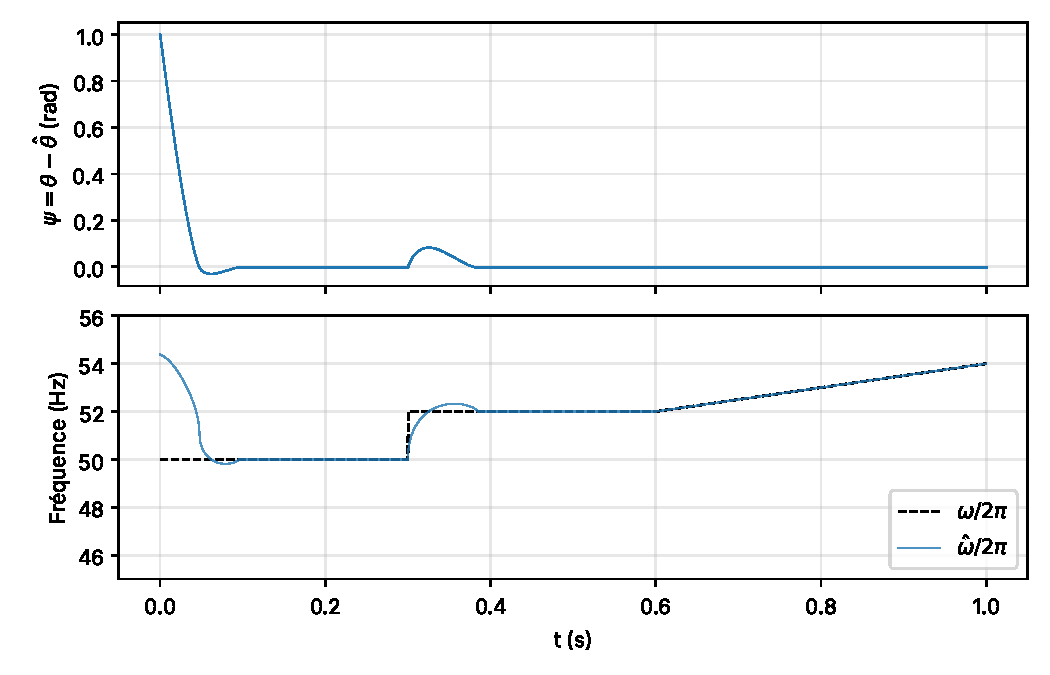
\includegraphics[width=0.85\textwidth]{figures/sim_pll_sta.pdf}
\caption{Simulation : $\psi(0)=1$ rad, puis un saut de fréquence de $+2$ Hz à $t=0.3$ s
et une rampe de $5$ Hz/s à partir de $t=0.6$ s ($k_1=30$, $k_2=150$).}
\end{figure}

\subsection{Limites de l'analyse}
\begin{itemize}
  \item \textbf{Saut de fréquence.} Un saut de $\omega$ ne respecte pas H2. Il se traduit
        par un saut de $x_2$. La convergence reste garantie si l'état après le saut est encore dans $\Omega_c$.
  \item \textbf{Déséquilibre et harmoniques.} La séquence inverse ajoute à $e$ une oscillation à
        $2\omega$, qui ne s'annule pas à l'équilibre. On obtient alors seulement une stabilité
        \emph{pratique} : $\psi$ reste dans un voisinage borné de $0$. Un pré-filtrage
        (DSOGI, MAF, etc.) est recommandé.
  \item \textbf{Échantillonnage.} Avec une période $T_s$, la précision du super-twisting est
        $|\psi| = O(T_s^2)$ et $|x_2| = O(T_s)$ (Levant). Il faut ajouter le retard de calcul
        d'un échantillon, $\approx\omega T_s$ (visible en simulation : $\approx3\cdot10^{-3}$ rad pour $T_s=10^{-5}$ s).
  \item \textbf{Normalisation.} Sans division par $\hat V_m$, les gains effectifs valent
        $k_1\sqrt{V_m}$ et $k_2$ reste inchangé. La condition \eqref{eq:k2} doit alors être vérifiée
        pour la plus petite amplitude envisagée (creux de tension).
\end{itemize}


\section{Résumé de l'algorithme}
\begin{enumerate}
  \item Mesurer $V_a,V_b,V_c$ et calculer $V_\alpha,V_\beta$ (Clarke).
  \item $\hat V_m=\sqrt{V_\alpha^2+V_\beta^2}$, \quad
        $e = \dfrac{-V_\alpha\sin\hth + V_\beta\cos\hth}{\hat V_m}$.
  \item $\hw = k_1|e|^{1/2}\sign(e) + z + \omega_{ff}$, \quad $\dot z = k_2\sign(e)$.
  \item $\dot\hth = \hw$ (intégration modulo $2\pi$).
\end{enumerate}

\begin{thebibliography}{9}
\bibitem{moreno} J.~A.~Moreno, M.~Osorio, ``A Lyapunov approach to second-order sliding mode controllers and observers,'' \emph{IEEE CDC}, 2008.
\bibitem{moreno12} J.~A.~Moreno, M.~Osorio, ``Strict Lyapunov functions for the super-twisting algorithm,'' \emph{IEEE TAC}, 57(4), 2012.
\bibitem{levant} A.~Levant, ``Sliding order and sliding accuracy in sliding mode control,'' \emph{Int. J. Control}, 58(6), 1993.
\end{thebibliography}

\end{document}
